% =====================================================================
%  Capítulo 15. Estructura temporal de las tasas de interés
% =====================================================================
\chapter[Estructura temporal de tasas]{Estructura temporal de las tasas de interés: expectativas, Nelson-Siegel y Vasicek}\label{cap:tasas}

\section*{Objetivos de aprendizaje}
Al terminar este capítulo, el lector podrá:
\begin{enumerate}[label=\arabic*.,leftmargin=*]
  \item Pasar entre precios de bonos cupón cero, rendimientos, tasas a plazo y rendimientos de mantener un bono, y
        demostrar las identidades que los unen.
  \item Contrastar la hipótesis de las expectativas con las regresiones de Campbell y Shiller y de Fama y Bliss, y
        entender por qué su rechazo implica primas por plazo variables.
  \item Resumir la curva con tres factores, ya sea estadísticos (componentes principales) o paramétricos (Nelson-Siegel
        en la versión dinámica de Diebold y Li).
  \item Estimar el modelo de Vasicek a partir de su discretización exacta y detectar el efecto nivel en la volatilidad
        (modelo CKLS).
\end{enumerate}

\section*{Motivación}
Un banco central fija la tasa a un día; los hogares y las empresas se endeudan a plazos de meses o de años. Lo que une
ambos extremos es la curva de rendimientos: la relación, en una fecha dada, entre el plazo de un bono y su
rendimiento. Su forma resume lo que el mercado espera de las tasas futuras y lo que cobra por cargar con el riesgo de
plazo. Una curva con pendiente negativa ha precedido a la mayoría de las recesiones de Estados Unidos desde la
posguerra, y los tesoreros, los fondos de pensiones y los reguladores la usan a diario para valorar flujos futuros.
Este capítulo trata la curva como un objeto econométrico: un vector de series de tiempo muy persistentes y muy
correlacionadas, con una estructura de factores fuerte y con restricciones teóricas que se pueden contrastar.

\paragraph{Datos del capítulo.} Rendimientos de bonos cupón cero del Tesoro de Estados Unidos, en porcentaje anual, a
fin de cada mes, de diciembre de 1946 a febrero de 1991 ($T=531$), para diez vencimientos: 1, 2, 3, 5, 6, 11, 12, 36, 60
y 120 meses. Son las curvas estimadas por McCulloch y Kwon (1993) a partir de precios de bonos con cupón, distribuidas en
la colección \texttt{Rdatasets} (conjunto \texttt{Irates} del paquete \texttt{Ecdat}). Es la misma clase de datos que usan
Campbell y Shiller (1991). En el texto los tratamos como rendimientos compuestos en forma continua. Para la curva soberana
peruana, el BCRP publica rendimientos por plazo que permiten repetir los ejercicios (Ejercicio propuesto 15.7).

% ---------------------------------------------------------------------
\section{Precios, rendimientos y tasas a plazo}
% ---------------------------------------------------------------------

Sea $P_{n,t}$ el precio en $t$ de un bono cupón cero que paga una unidad dentro de $n$ períodos. Su rendimiento
(compuesto en forma continua, por período) $y_{n,t}$ es la tasa constante que descuenta ese pago al precio de mercado:
\[
  P_{n,t}=e^{-n\,y_{n,t}},\qquad y_{n,t}=-\frac{1}{n}\ln P_{n,t}.
\]
La \emph{curva de rendimientos} en la fecha $t$ es la función $n\mapsto y_{n,t}$. Con $p_{n,t}=\ln P_{n,t}$ escribimos
$p_{n,t}=-n\,y_{n,t}$.

\begin{definicion}[Tasa a plazo]
La tasa a plazo $f_t(n,m)$, con $n<m$, es la tasa que hoy se puede asegurar para prestar entre $t+n$ y $t+m$. La tasa a
plazo de un período que empieza en $t+n-1$ se escribe $f_t(n)=f_t(n-1,n)$.
\end{definicion}

\begin{proposicion}[Tasa a plazo implícita]\label{prop:plazo}
En ausencia de arbitraje,
\[
  f_t(n,m)=\frac{m\,y_{m,t}-n\,y_{n,t}}{m-n},\qquad f_t(n)=n\,y_{n,t}-(n-1)\,y_{n-1,t}.
\]
\end{proposicion}

\begin{proof}
Hay dos formas de llevar una unidad de hoy hasta $t+m$. La primera es comprar bonos de $m$ períodos. La segunda es
comprar bonos de $n$ períodos y, al mismo tiempo, pactar hoy un préstamo a la tasa $f_t(n,m)$ entre $t+n$ y $t+m$.
Ambas estrategias no tienen riesgo, así que deben rendir lo mismo:
\begin{align*}
  e^{m\,y_{m,t}} &= e^{n\,y_{n,t}}\,e^{(m-n)f_t(n,m)}\\
  m\,y_{m,t}     &= n\,y_{n,t}+(m-n)\,f_t(n,m)\\
  (m-n)\,f_t(n,m) &= m\,y_{m,t}-n\,y_{n,t}\\
  f_t(n,m)       &= \frac{m\,y_{m,t}-n\,y_{n,t}}{m-n}.
\end{align*}
Para la tasa de un período, tomamos $m=n$ y $n-1$ en lugar de $n$:
\begin{align*}
  f_t(n) &= \frac{n\,y_{n,t}-(n-1)\,y_{n-1,t}}{n-(n-1)}\\
         &= n\,y_{n,t}-(n-1)\,y_{n-1,t}.
\end{align*}
\end{proof}

La fórmula también dice que el rendimiento es el promedio de las tasas a plazo de un período:
\[
  y_{n,t}=\frac1n\sum_{i=1}^{n}f_t(i),\qquad f_t(1)=y_{1,t},
\]
pues la suma de $f_t(i)=i\,y_{i,t}-(i-1)\,y_{i-1,t}$ es telescópica. Cuando la curva sube, las tasas a plazo están por encima
de los rendimientos; cuando baja, por debajo.

\begin{definicion}[Rendimiento de mantener un bono]
El rendimiento logarítmico de comprar en $t$ un bono de $n$ períodos y venderlo en $t+1$, cuando le quedan $n-1$, es
$h_{t+1}(n)=p_{n-1,t+1}-p_{n,t}$. Su exceso sobre la tasa de un período es $rx_{t+1}(n)=h_{t+1}(n)-y_{1,t}$.
\end{definicion}

\begin{proposicion}[Descomposición del rendimiento en exceso]\label{prop:rx}
\[
  rx_{t+1}(n)=\bigl[f_t(n)-y_{1,t}\bigr]-(n-1)\bigl[y_{n-1,t+1}-y_{n-1,t}\bigr].
\]
\end{proposicion}

\begin{proof}
Partimos de la definición y sustituimos $p=-n\,y$:
\begin{align*}
  rx_{t+1}(n) &= p_{n-1,t+1}-p_{n,t}-y_{1,t}\\
              &= -(n-1)\,y_{n-1,t+1}+n\,y_{n,t}-y_{1,t}.
\end{align*}
Sumamos y restamos $(n-1)\,y_{n-1,t}$:
\begin{align*}
  rx_{t+1}(n) &= n\,y_{n,t}-(n-1)\,y_{n-1,t}-y_{1,t}-(n-1)\,y_{n-1,t+1}+(n-1)\,y_{n-1,t}\\
              &= \bigl[f_t(n)-y_{1,t}\bigr]-(n-1)\bigl[y_{n-1,t+1}-y_{n-1,t}\bigr],
\end{align*}
donde el último paso usa la Proposición~\ref{prop:plazo}.
\end{proof}

El rendimiento en exceso tiene una parte conocida en $t$, el diferencial entre la tasa a plazo y la tasa corta, y una
parte aleatoria: la pérdida de capital si el rendimiento sube. El factor $(n-1)$ es la duración del bono al venderlo; por
eso los bonos largos son mucho más volátiles que los cortos.

% ---------------------------------------------------------------------
\section{La hipótesis de las expectativas}
% ---------------------------------------------------------------------

La hipótesis de las expectativas (HE) afirma que los rendimientos largos son el promedio de las tasas cortas esperadas,
más una prima por plazo que puede depender del vencimiento pero \emph{no del tiempo}:
\[
  y_{n,t}=\frac1n\sum_{i=0}^{n-1}\E_t\bigl[y_{1,t+i}\bigr]+c_n .
\]
Una forma equivalente es que el rendimiento en exceso esperado de cualquier bono es constante:
$\E_t[rx_{t+1}(n)]=\text{constante}$. La HE tiene tres implicaciones contrastables.

\begin{proposicion}[Tasas cortas futuras]\label{prop:he1}
Sea $k=hm$, con $h$ entero. Bajo la HE, en la regresión
\[
  \frac1h\sum_{i=0}^{h-1}y_{m,t+mi}-y_{m,t}=a+b\,\bigl(y_{k,t}-y_{m,t}\bigr)+u_{t+k-m},
\]
el coeficiente poblacional es $b=1$.
\end{proposicion}

\begin{proof}
Aplicada a bonos de $k$ períodos y de $m$ períodos que se renuevan $h$ veces, la HE dice que
$y_{k,t}=\frac1h\sum_{i=0}^{h-1}\E_t[y_{m,t+mi}]+c$, con $c$ constante. Llamemos $Z_t$ al lado izquierdo de la regresión y
$S_t=y_{k,t}-y_{m,t}$ a la pendiente. Entonces
\begin{align*}
  \E_t[Z_t] &= \frac1h\sum_{i=0}^{h-1}\E_t[y_{m,t+mi}]-y_{m,t}\\
            &= y_{k,t}-c-y_{m,t}\\
            &= S_t-c .
\end{align*}
El error de predicción $u_t=Z_t-\E_t[Z_t]$ no está correlacionado con nada conocido en $t$, y $S_t$ se conoce en $t$. Por
tanto,
\begin{align*}
  \Cov(Z_t,S_t) &= \Cov\bigl(\E_t[Z_t]+u_t,\ S_t\bigr)\\
                &= \Cov(S_t-c,\ S_t)+\Cov(u_t,S_t)\\
                &= \Var(S_t)+0,
\end{align*}
y el coeficiente de MCO en la población es $b=\Cov(Z_t,S_t)/\Var(S_t)=1$.
\end{proof}

\begin{proposicion}[Regresión de la tasa larga de Campbell y Shiller]\label{prop:he2}
Bajo la HE, en la regresión
\[
  y_{n-1,t+1}-y_{n,t}=a+b\,\frac{y_{n,t}-y_{1,t}}{n-1}+u_{t+1}
\]
el coeficiente poblacional es $b=1$: cuando la curva tiene pendiente positiva, el rendimiento largo debe \emph{subir}.
\end{proposicion}

\begin{proof}
La HE con primas constantes implica que el rendimiento de mantener el bono largo un período iguala, en esperanza, a la
tasa corta más una constante: $\E_t[h_{t+1}(n)]=y_{1,t}+c$. Usando $h_{t+1}(n)=n\,y_{n,t}-(n-1)\,y_{n-1,t+1}$:
\begin{align*}
  n\,y_{n,t}-(n-1)\,\E_t[y_{n-1,t+1}] &= y_{1,t}+c\\
  (n-1)\,\E_t[y_{n-1,t+1}]            &= n\,y_{n,t}-y_{1,t}-c\\
  \E_t[y_{n-1,t+1}]-y_{n,t}           &= \frac{n\,y_{n,t}-y_{1,t}-c}{n-1}-\frac{(n-1)\,y_{n,t}}{n-1}\\
                                      &= \frac{y_{n,t}-y_{1,t}}{n-1}-\frac{c}{n-1}.
\end{align*}
Igual que en la proposición anterior, el error de predicción no está correlacionado con la pendiente, y el coeficiente
es $b=1$.
\end{proof}

La intuición es la de un arbitraje: si el bono largo rinde más que el corto por su cupón implícito, la única forma de
que ambos tengan el mismo rendimiento esperado es que el largo sufra una pérdida de capital, es decir, que su rendimiento
suba.

\begin{corolario}[Regresión de Fama y Bliss]\label{cor:fb}
Bajo la HE, en la regresión $rx_{t+1}(n)=a+b\,[f_t(n)-y_{1,t}]+u_{t+1}$ el coeficiente es $b=0$.
\end{corolario}

\begin{proof}
Bajo la HE, $\E_t[rx_{t+1}(n)]$ es una constante. Una constante no está correlacionada con ninguna variable conocida en
$t$, en particular con el diferencial a plazo:
\begin{align*}
  \Cov\bigl(rx_{t+1}(n),\ f_t(n)-y_{1,t}\bigr) &= \Cov\bigl(\E_t[rx_{t+1}(n)]+u_{t+1},\ f_t(n)-y_{1,t}\bigr)\\
                                               &= 0+0 .
\end{align*}
\end{proof}

Las tres regresiones son caras de la misma hipótesis. Por la Proposición~\ref{prop:rx}, si en la de Campbell y Shiller el
coeficiente es menor que uno, el rendimiento largo no sube lo suficiente, el bono largo rinde más cuando la pendiente es
alta y en la de Fama y Bliss el coeficiente es positivo. En ambos casos la conclusión es que la prima por plazo
\emph{varía en el tiempo} y es predecible con la forma de la curva.

\begin{observacion}
Cuando el horizonte $k$ es mayor que la frecuencia de los datos, los lados izquierdos de meses consecutivos comparten
$k-m$ observaciones: los errores siguen un MA$(k-m)$ incluso bajo la hipótesis nula. Por eso se usan errores estándar de
Newey-West con al menos $k-m$ rezagos (Capítulo~\ref{cap:robustos}). Además, las regresiones de pendiente sufren un sesgo
de muestra finita, porque el regresor es muy persistente; con horizontes de diez años y 44 años de datos hay apenas cuatro
observaciones independientes.
\end{observacion}

% ---------------------------------------------------------------------
\section{Modelos de factores de la curva}
% ---------------------------------------------------------------------

Diez rendimientos que se mueven casi juntos son una matriz de covarianzas casi de rango bajo. Litterman y Scheinkman
(1991) mostraron que tres componentes principales, a los que llamaron \emph{nivel}, \emph{pendiente} y \emph{curvatura},
explican más del 95\,\% de la variación de los rendimientos. El Ejercicio~\ref{ej:curva} lo verifica.

\subsection*{Nelson-Siegel}
Nelson y Siegel (1987) propusieron una forma paramétrica para la curva en una fecha:
\[
  y(\tau)=\beta_0+\beta_1\,\frac{1-e^{-\lambda\tau}}{\lambda\tau}
          +\beta_2\Bigl(\frac{1-e^{-\lambda\tau}}{\lambda\tau}-e^{-\lambda\tau}\Bigr).
\]
Diebold y Li (2006) la volvieron dinámica: fijan $\lambda$ y dejan que los tres coeficientes varíen cada mes,
$\boldsymbol\beta_t=(\beta_{0t},\beta_{1t},\beta_{2t})'$. Con $\lambda$ fijo, la curva es lineal en $\boldsymbol\beta_t$, que se
estima por MCO de corte transversal fecha por fecha.

\begin{proposicion}[Interpretación de las cargas]\label{prop:ns}
Para $\lambda>0$:
\begin{enumerate}[label=(\alph*)]
  \item $\displaystyle\lim_{\tau\to\infty}y(\tau)=\beta_0$: $\beta_0$ es el nivel de largo plazo.
  \item $\displaystyle\lim_{\tau\to0}y(\tau)=\beta_0+\beta_1$: la tasa instantánea; $-\beta_1$ es la pendiente
        (largo menos corto).
  \item La carga de $\beta_2$ vale cero en ambos extremos y tiene un único máximo en $\lambda\tau=x^*\approx1{,}7933$.
\end{enumerate}
\end{proposicion}

\begin{proof}
Escribimos $x=\lambda\tau$ y $s(x)=(1-e^{-x})/x$.

(a) Cuando $x\to\infty$, $e^{-x}\to0$:
\begin{align*}
  s(x) &= \frac{1-e^{-x}}{x}\ \to\ \frac{1-0}{\infty}=0,\\
  s(x)-e^{-x} &\to 0-0=0,\\
  y(\tau) &\to \beta_0+\beta_1\cdot0+\beta_2\cdot0=\beta_0 .
\end{align*}

(b) Cuando $x\to0$, usamos $e^{-x}=1-x+\frac{x^2}{2}+O(x^3)$:
\begin{align*}
  1-e^{-x} &= x-\frac{x^2}{2}+O(x^3)\\
  s(x)     &= 1-\frac{x}{2}+O(x^2)\ \to\ 1,\\
  s(x)-e^{-x} &\to 1-1=0,\\
  y(\tau)  &\to \beta_0+\beta_1\cdot1+\beta_2\cdot0=\beta_0+\beta_1 .
\end{align*}

(c) Sea $g(x)=s(x)-e^{-x}$. Por (a) y (b), $g(x)\to0$ en ambos extremos, y $g(x)>0$ para $x>0$ porque
$1-e^{-x}>x\,e^{-x}$ (equivale a $e^{x}>1+x$). Su derivada es
\begin{align*}
  g'(x) &= \frac{x\,e^{-x}-(1-e^{-x})}{x^2}+e^{-x}\\
        &= \frac{x\,e^{-x}-1+e^{-x}+x^2e^{-x}}{x^2}\\
        &= \frac{e^{-x}\,(x^2+x+1)-1}{x^2}.
\end{align*}
El numerador $q(x)=e^{-x}(x^2+x+1)-1$ vale cero en $x=0$ y su derivada es
\begin{align*}
  q'(x) &= -e^{-x}(x^2+x+1)+e^{-x}(2x+1)\\
        &= e^{-x}\,(x-x^2)\\
        &= e^{-x}\,x\,(1-x),
\end{align*}
positiva en $(0,1)$ y negativa en $(1,\infty)$. Así $q$ sube desde cero hasta $x=1$ y luego decrece hacia $-1$: cruza el
cero una sola vez, en $x^*>1$. Ese cruce es el único punto crítico de $g$, y como $g$ es positiva y se anula en los
extremos, es un máximo. Numéricamente, $x^*=1{,}7933$.
\end{proof}

Diebold y Li eligen $\lambda=0{,}0609$ (con $\tau$ en meses) para que la carga de curvatura sea máxima en
$\tau=1{,}7933/0{,}0609=29{,}45$ meses, entre los dos y los tres años. La Figura~\ref{fig:ns} muestra las tres cargas y las
formas de curva que generan: con $\beta_1<0$ la curva sube, con $\beta_1>0$ se invierte y con $\beta_2>0$ aparece una
joroba en los plazos medios.

\begin{figure}[ht]
\centering
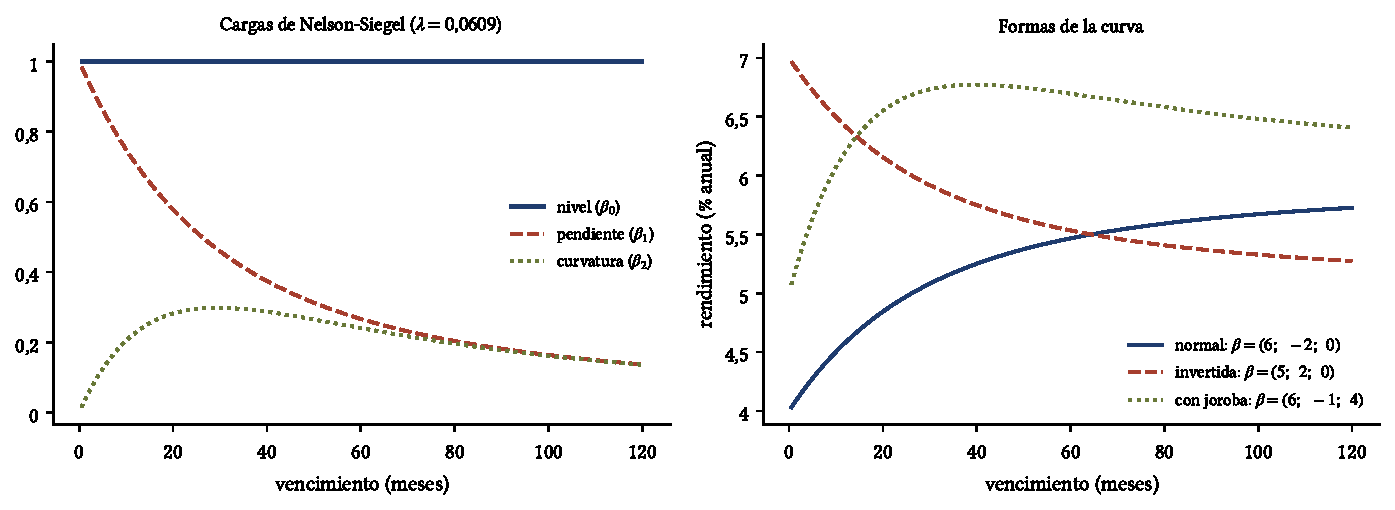
\includegraphics[width=\linewidth]{graficos/cap15_fig_nelson_siegel.pdf}
\caption{Izquierda: cargas de Nelson-Siegel con $\lambda=0{,}0609$. La de nivel es constante, la de pendiente cae de 1 a 0
y la de curvatura alcanza su máximo, 0,2984, en $\tau=29{,}45$ meses. Derecha: tres curvas generadas con distintos
$\boldsymbol\beta$.}
\label{fig:ns}
\end{figure}

\begin{observacion}
La versión de Diebold y Li no impone la ausencia de arbitraje entre vencimientos. Christensen, Diebold y Rudebusch
(2011) muestran que agregar un pequeño término de ajuste por convexidad la vuelve libre de arbitraje sin perder su
ajuste. Para pronosticar, Diebold y Li modelan cada $\beta_{jt}$ como un AR(1), algo que solo tiene sentido si los factores
son persistentes, como se verifica en el Ejercicio~\ref{ej:ns}.
\end{observacion}

% ---------------------------------------------------------------------
\section{Modelos de la tasa corta: Vasicek y CKLS}
% ---------------------------------------------------------------------

Los modelos de equilibrio parten de la dinámica de la tasa instantánea $r_t$. Vasicek (1977) propuso un proceso de
Ornstein-Uhlenbeck:
\[
  dr_t=\kappa(\theta-r_t)\,dt+\sigma\,dW_t,\qquad \kappa>0 .
\]
La tasa vuelve hacia $\theta$ con una velocidad proporcional a la distancia, y $\sigma$ es la volatilidad.

\begin{proposicion}[Discretización exacta de Vasicek]\label{prop:vasicek}
Para un intervalo $\Delta>0$,
\[
  r_{t+\Delta}=\theta+e^{-\kappa\Delta}(r_t-\theta)+\varepsilon_{t+\Delta},\qquad
  \varepsilon_{t+\Delta}\sim N\!\Bigl(0,\ \sigma^2\,\frac{1-e^{-2\kappa\Delta}}{2\kappa}\Bigr),
\]
y los $\varepsilon$ de intervalos disjuntos son independientes. Es decir, $r$ muestreado cada $\Delta$ es un AR(1)
$r_{t+\Delta}=a+b\,r_t+\varepsilon$ con
\[
  b=e^{-\kappa\Delta},\qquad a=\theta(1-b),\qquad \Var(\varepsilon)=s^2=\sigma^2\,\frac{1-b^2}{2\kappa}.
\]
\end{proposicion}

\begin{proof}
Sea $Z_t=e^{\kappa t}(r_t-\theta)$. Por el lema de Itô, como $Z$ es lineal en $r$:
\begin{align*}
  dZ_t &= \kappa e^{\kappa t}(r_t-\theta)\,dt+e^{\kappa t}\,dr_t\\
       &= \kappa e^{\kappa t}(r_t-\theta)\,dt+e^{\kappa t}\bigl[\kappa(\theta-r_t)\,dt+\sigma\,dW_t\bigr]\\
       &= \kappa e^{\kappa t}(r_t-\theta)\,dt-\kappa e^{\kappa t}(r_t-\theta)\,dt+\sigma e^{\kappa t}\,dW_t\\
       &= \sigma e^{\kappa t}\,dW_t .
\end{align*}
Integramos entre $t$ y $t+\Delta$:
\begin{align*}
  Z_{t+\Delta}-Z_t &= \sigma\int_t^{t+\Delta}e^{\kappa u}\,dW_u\\
  e^{\kappa(t+\Delta)}(r_{t+\Delta}-\theta) &= e^{\kappa t}(r_t-\theta)+\sigma\int_t^{t+\Delta}e^{\kappa u}\,dW_u\\
  r_{t+\Delta}-\theta &= e^{-\kappa\Delta}(r_t-\theta)+\sigma\int_t^{t+\Delta}e^{-\kappa(t+\Delta-u)}\,dW_u .
\end{align*}
El último término es una integral de Itô de una función determinista: es normal, con media cero, independiente de lo
ocurrido antes de $t$, y por la isometría de Itô su varianza es
\begin{align*}
  \Var(\varepsilon_{t+\Delta}) &= \sigma^2\int_t^{t+\Delta}e^{-2\kappa(t+\Delta-u)}\,du\\
                               &= \sigma^2\int_0^{\Delta}e^{-2\kappa v}\,dv\\
                               &= \sigma^2\,\Bigl[-\frac{e^{-2\kappa v}}{2\kappa}\Bigr]_0^{\Delta}\\
                               &= \sigma^2\,\frac{1-e^{-2\kappa\Delta}}{2\kappa}.
\end{align*}
Para la forma AR(1), expandimos:
\begin{align*}
  r_{t+\Delta} &= \theta+b\,r_t-b\,\theta+\varepsilon_{t+\Delta}\\
               &= \theta(1-b)+b\,r_t+\varepsilon_{t+\Delta},
\end{align*}
con $b=e^{-\kappa\Delta}$ y $b^2=e^{-2\kappa\Delta}$.
\end{proof}

\begin{corolario}[Del AR(1) a Vasicek]\label{cor:vasicek}
Dados los estimadores $\hat a$, $\hat b\in(0,1)$ y $\hat s$ del AR(1),
\[
  \hat\kappa=-\frac{\ln\hat b}{\Delta},\qquad \hat\theta=\frac{\hat a}{1-\hat b},\qquad
  \hat\sigma=\hat s\sqrt{\frac{2\hat\kappa}{1-\hat b^2}} .
\]
La vida media de una desviación de $\theta$ es $\ln2/\kappa$, y la distribución estacionaria es
$N\bigl(\theta,\ \sigma^2/(2\kappa)\bigr)$.
\end{corolario}

\begin{proof}
Las tres fórmulas se obtienen despejando la Proposición~\ref{prop:vasicek}. La vida media es el $\Delta$ que reduce a la
mitad la desviación esperada:
\begin{align*}
  e^{-\kappa\Delta} &= \tfrac12\\
  -\kappa\Delta     &= -\ln 2\\
  \Delta            &= \ln2/\kappa .
\end{align*}
La varianza estacionaria $v$ resuelve $v=b^2v+s^2$:
\begin{align*}
  v &= \frac{s^2}{1-b^2}\\
    &= \frac{\sigma^2(1-b^2)}{2\kappa(1-b^2)}\\
    &= \frac{\sigma^2}{2\kappa}.
\end{align*}
\end{proof}

Como la discretización es exacta, la máxima verosimilitud del AR(1) gaussiano (que coincide con MCO condicionando en la
primera observación) es la máxima verosimilitud de Vasicek. La Figura~\ref{fig:vasicek} muestra trayectorias que parten de
1, 5 y 10\,\% con $\kappa=0{,}5$, $\theta=5$ y $\sigma=1$: la vida media es $\ln2/0{,}5=1{,}386$ años y la desviación
estándar estacionaria, $1/\sqrt{2\times0{,}5}=1$.

\begin{figure}[ht]
\centering
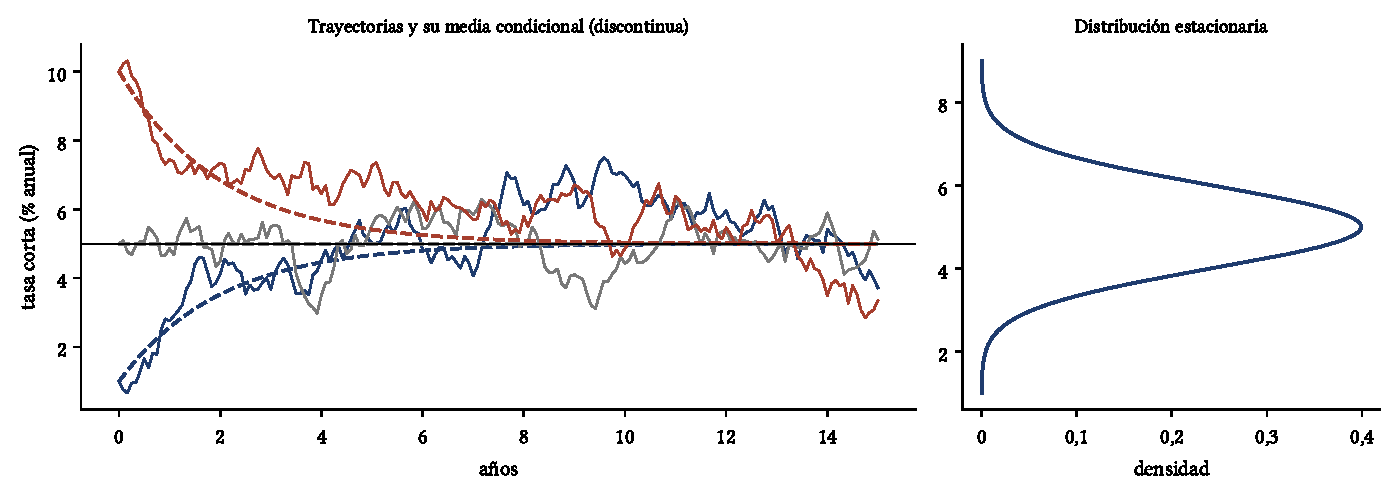
\includegraphics[width=\linewidth]{graficos/cap15_fig_vasicek.pdf}
\caption{Modelo de Vasicek con $\kappa=0{,}5$, $\theta=5$ y $\sigma=1$, simulado mes a mes con la discretización exacta.
Izquierda: tres trayectorias y su media condicional $\theta+(r_0-\theta)e^{-\kappa t}$. Derecha: distribución estacionaria
$N(5;\,1)$, que asigna una probabilidad positiva a tasas negativas.}
\label{fig:vasicek}
\end{figure}

\paragraph{El modelo CKLS.} En Vasicek la volatilidad no depende del nivel, y la tasa puede volverse negativa. Chan,
Karolyi, Longstaff y Sanders (1992) anidan varios modelos en
\[
  dr_t=(\alpha+\beta r_t)\,dt+\sigma\,r_t^{\gamma}\,dW_t ,
\]
donde $\gamma=0$ es Vasicek, $\gamma=1/2$ es Cox, Ingersoll y Ross (1985) y $\gamma=1$ es un movimiento browniano
geométrico con reversión. Con un paso pequeño, $\Var(\varepsilon_{t+\Delta}\mid r_t)\approx\sigma^2r_t^{2\gamma}\Delta$, de modo que
\[
  \ln\varepsilon_{t+\Delta}^2\approx\ln(\sigma^2\Delta)+2\gamma\ln r_t+\ln\eta^2_{t+\Delta},
\]
con $\eta$ normal estándar. Una regresión del logaritmo del residuo al cuadrado sobre el logaritmo del nivel estima $2\gamma$
de forma simple. CKLS estimaron $\gamma\approx1{,}5$ por MGM con la tasa a un mes de 1964 a 1989.

% ---------------------------------------------------------------------
\section{Ejercicios resueltos}
% ---------------------------------------------------------------------

\begin{ejresuelto}{Hechos estilizados de la curva}\label{ej:curva}
\enunciado Describa los diez rendimientos: medias, volatilidades, persistencia y correlaciones. Calcule la pendiente
$y_{120}-y_3$ y cuente los meses con curva invertida. Extraiga los componentes principales de la matriz de covarianzas e
interprételos.

\solucion
\paso{Paso 1. Estadísticas descriptivas.}
\begin{center}\small
\begin{tabular}{@{}rrrrrr@{}}
\toprule
Vencimiento (meses) & Media & Desv.\ est. & $\hat\rho(1)$ & $\hat\rho(12)$ & Corr.\ con 1 mes \\
\midrule
1   & 4,820 & 3,193 & 0,9800 & 0,8260 & 1,0000 \\
3   & 5,126 & 3,285 & 0,9844 & 0,8382 & 0,9963 \\
12  & 5,526 & 3,354 & 0,9862 & 0,8617 & 0,9853 \\
36  & 5,821 & 3,302 & 0,9900 & 0,8935 & 0,9624 \\
60  & 5,973 & 3,267 & 0,9918 & 0,9056 & 0,9492 \\
120 & 6,157 & 3,188 & 0,9937 & 0,9204 & 0,9329 \\
\bottomrule
\end{tabular}
\end{center}
La curva \emph{media} sube: de 4,82\,\% a un mes a 6,16\,\% a diez años. La volatilidad casi no cambia con el plazo. Todos
los rendimientos son muy persistentes (autocorrelación mensual de 0,98 a 0,99, más alta cuanto más largo el plazo) y están
muy correlacionados entre sí, aunque la correlación cae con la distancia entre vencimientos.

\paso{Paso 2. La pendiente.} La pendiente $y_{120}-y_3$ tiene una media de $1{,}032$ puntos porcentuales. La curva estuvo
invertida en 63 de 531 meses (11,9\,\%). El mínimo, $-3{,}223$, ocurrió en marzo de 1980, durante el endurecimiento monetario
de Volcker; el máximo, $4{,}108$, en agosto de 1982, cuando la política se relajó y las tasas cortas cayeron primero.

\paso{Paso 3. Componentes principales.} Los tres primeros explican el 98,25\,\%, el 1,54\,\% y el 0,15\,\% de la varianza
total (99,94\,\% en conjunto). Sus cargas:
\begin{center}\small
\begin{tabular}{@{}rrrr@{}}
\toprule
Vencimiento & CP1 & CP2 & CP3 \\
\midrule
1   & 0,306 & $-0{,}316$ & 0,527 \\
3   & 0,317 & $-0{,}267$ & 0,148 \\
6   & 0,323 & $-0{,}184$ & $-0{,}239$ \\
12  & 0,325 & $-0{,}019$ & $-0{,}423$ \\
36  & 0,318 & 0,334 & $-0{,}146$ \\
60  & 0,312 & 0,464 & 0,073 \\
120 & 0,300 & 0,576 & 0,374 \\
\bottomrule
\end{tabular}
\end{center}
El primero carga casi igual en todos los plazos (0,30 a 0,325): mueve toda la curva en paralelo, es el \emph{nivel}. El
segundo crece de forma monótona con el plazo, de $-0{,}316$ a $0{,}576$: inclina la curva, es la \emph{pendiente}. El
tercero es positivo en los extremos y negativo en los plazos de 6 a 36 meses: dobla la curva, es la \emph{curvatura}. Es el
patrón de Litterman y Scheinkman (Figura~\ref{fig:curvas}).

\codigoweb{cap15_ej01}
\salidaR{cap15_ej01_R.txt}
\lectura{cap15_ej01}

\RvsPy El signo de los autovectores es arbitrario y \texttt{eigen} (R) y \texttt{np.linalg.eigh} (Python) no siempre coinciden.
Fijamos cada signo para que la carga a 120 meses sea positiva. \texttt{eigh} devuelve los autovalores de menor a mayor, así
que en Python se invierte el orden. Las autocorrelaciones salen de \texttt{acf} en R y de
\texttt{statsmodels.tsa.stattools.acf} en Python, que usan la misma definición (sumas centradas divididas entre la suma
total de cuadrados).

\begin{figure}[ht]
\centering
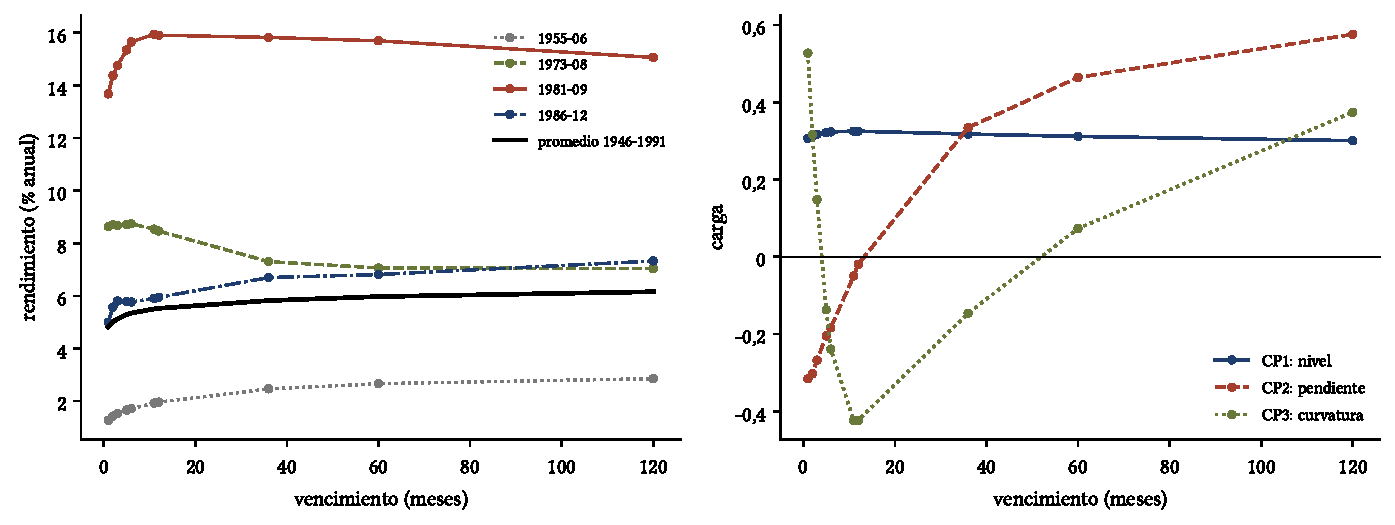
\includegraphics[width=\linewidth]{graficos/cap15_ej01_curvas_cp.pdf}
\caption{Izquierda: curvas observadas en cuatro fechas y la curva media de 1946 a 1991. En septiembre de 1981 la curva tiene joroba:
sube de 13,7\,\% a un mes a 15,9\,\% a 11 meses y baja a 15,1\,\% a diez años. Derecha: cargas de los tres primeros componentes principales: nivel, pendiente y curvatura.}
\label{fig:curvas}
\end{figure}

\begin{conclusion}
La curva de rendimientos es, en la práctica, un objeto de tres dimensiones. El nivel explica casi toda la varianza, pero la
pendiente y la curvatura, aunque pequeñas, son las que contienen información sobre expectativas y primas por plazo.
\end{conclusion}
\end{ejresuelto}

\begin{ejresuelto}{La hipótesis de las expectativas}\label{ej:he}
\enunciado Contraste la HE con (a) la regresión de tasas cortas futuras de la Proposición~\ref{prop:he1}, para
$(m,k)=(1,3),(1,6),(1,12)$ con datos mensuales y $(12,36),(12,60),(12,120)$ renovando bonos de un año, con errores de
Newey-West de $k$ rezagos; y (b) la regresión de la tasa larga de la Proposición~\ref{prop:he2} con $n=12$ meses.

\solucion
\paso{Paso 1. Tasas cortas futuras.} Para $(m,k)=(1,3)$, el lado izquierdo es el promedio de la tasa a un mes en
$t$, $t+1$ y $t+2$ menos la tasa de hoy, y el regresor es $y_{3,t}-y_{1,t}$. Se pierden $k-m=2$ observaciones al final.
\begin{center}\small
\begin{tabular}{@{}rrrrrrr@{}}
\toprule
$m$ & $k$ & $n$ & $\hat b$ & ee($\hat b$) & $t(b=1)$ & $R^2$ \\
\midrule
1  & 3   & 529 & 0,4447 & 0,1381 & $-4{,}02$ & 0,082 \\
1  & 6   & 526 & 0,2928 & 0,1429 & $-4{,}95$ & 0,030 \\
1  & 12  & 520 & 0,2468 & 0,1738 & $-4{,}33$ & 0,022 \\
12 & 36  & 507 & 0,2000 & 0,3928 & $-2{,}04$ & 0,007 \\
12 & 60  & 483 & 0,5566 & 0,3969 & $-1{,}12$ & 0,061 \\
12 & 120 & 423 & 1,5406 & 0,2580 & 2,10 & 0,519 \\
\bottomrule
\end{tabular}
\end{center}
Para $(1,3)$, el estadístico es
\begin{align*}
  t &= \frac{0{,}4447-1}{0{,}1381}\\
    &= \frac{-0{,}5553}{0{,}1381}\\
    &= -4{,}02 .
\end{align*}
En el extremo corto los coeficientes son positivos, la pendiente sí predice la dirección de las tasas, pero muy por
debajo de uno: la HE se rechaza con claridad. A horizontes largos el coeficiente sube y a diez años supera a uno, el patrón
en forma de U que documentaron Campbell y Shiller (1991). Con 423 observaciones solapadas a diez años hay pocas
observaciones independientes y el resultado debe leerse con cautela.

\paso{Paso 2. La tasa larga.} Con $n=12$, el lado izquierdo es $y_{11,t+1}-y_{12,t}$ y el regresor $(y_{12,t}-y_{1,t})/11$:
\begin{align*}
  \hat b &= -1{,}3515 \quad(\text{ee }0{,}6210),\\
  t(b=1) &= \frac{-1{,}3515-1}{0{,}6210}\\
         &= \frac{-2{,}3515}{0{,}6210}\\
         &= -3{,}79 .
\end{align*}
El coeficiente no solo es menor que uno: es \emph{negativo}. Cuando la curva sube, el rendimiento a un año tiende a bajar en
el mes siguiente, lo contrario de lo que exige la HE (Figura~\ref{fig:he}).

\codigoweb{cap15_ej02}
\salidaR{cap15_ej02_R.txt}
\lectura{cap15_ej02}

\RvsPy La función \texttt{mco\_nw} es nuestra en ambos lenguajes, para controlar el núcleo de Bartlett y el número de
rezagos. En Python, la opción \texttt{cov\_type="HAC"} de \texttt{statsmodels}, con
\texttt{cov\_kwds=\{"maxlags": k\}}, da los mismos errores (lo comprobamos en la regresión de la tasa larga: 0,6210). En R,
la función \texttt{NeweyWest} del paquete \texttt{sandwich}, con \texttt{prewhite = FALSE} y \texttt{adjust = FALSE}, usa
los mismos pesos. El
promedio de las tasas futuras se arma con índices $t+m\,i$; en R conviene \texttt{sapply}, en Python una comprensión de listas.

\begin{figure}[ht]
\centering
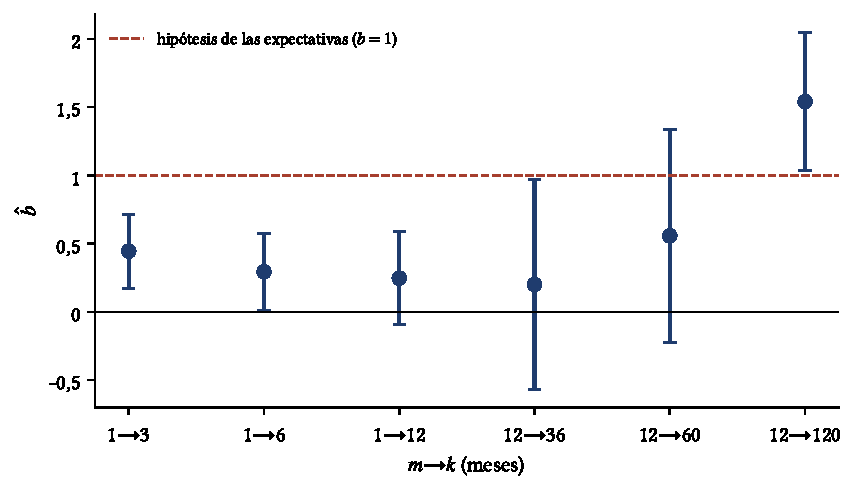
\includegraphics[width=0.8\linewidth]{graficos/cap15_ej02_expectativas.pdf}
\caption{Coeficientes de la regresión de tasas cortas futuras con intervalos al 95\,\% (Newey-West). La HE exige que todos
estén en la línea discontinua.}
\label{fig:he}
\end{figure}

\begin{conclusion}
La pendiente de la curva predice las tasas futuras en la dirección correcta, pero mucho menos de lo que exige la HE en el
corto plazo, y la tasa larga se mueve en sentido contrario. La explicación más aceptada es una prima por plazo que varía
en el tiempo y que hace que la pendiente mida, en parte, esa prima y no solo expectativas.
\end{conclusion}
\end{ejresuelto}

\begin{ejresuelto}{Rendimientos en exceso y Fama-Bliss}\label{ej:fb}
\enunciado Calcule los rendimientos en exceso a un mes de los bonos de 2, 3, 6 y 12 meses, sus medias y razones de Sharpe, y
estime la regresión de Fama y Bliss sobre el diferencial a plazo.

\solucion
\paso{Paso 1. Unidades.} Los rendimientos están en porcentaje anual y el período es un mes, así que la tasa por período es
$y/12$. Por la definición y la Proposición~\ref{prop:plazo}, en porcentaje mensual,
\begin{align*}
  rx_{t+1}(n) &= \frac{n}{12}\,y_{n,t}-\frac{n-1}{12}\,y_{n-1,t+1}-\frac{y_{1,t}}{12},\\
  \frac{f_t(n)-y_{1,t}}{12} &= \frac{n\,y_{n,t}-(n-1)\,y_{n-1,t}-y_{1,t}}{12}.
\end{align*}
Los vencimientos disponibles permiten $n-1=1,2,5,11$ para $n=2,3,6,12$.

\paso{Paso 2. Resultados.}
\begin{center}\small
\begin{tabular}{@{}rrrrrrrr@{}}
\toprule
$n$ & Media $rx$ & Desv.\ est. & Sharpe anual & $\hat b$ & ee & $t(b=0)$ & $R^2$ \\
\midrule
2  & 0,0302 & 0,0509 & 2,053 & 0,5159 & 0,0990 & 5,21 & 0,118 \\
3  & 0,0435 & 0,0964 & 1,563 & 0,6973 & 0,1958 & 3,56 & 0,091 \\
6  & 0,0641 & 0,2324 & 0,956 & 1,3023 & 0,3297 & 3,95 & 0,103 \\
12 & 0,0689 & 0,4882 & 0,489 & 1,1656 & 0,4836 & 2,41 & 0,035 \\
\bottomrule
\end{tabular}
\end{center}
Los bonos más largos rinden más en promedio: el de 12 meses rinde $0{,}0689\times12=0{,}83$ puntos porcentuales anuales más
que la letra a un mes. Pero su volatilidad crece más rápido, por el factor de duración $(n-1)$ de la
Proposición~\ref{prop:rx}, y la razón de Sharpe cae de 2,05 a 0,49.

\paso{Paso 3. Fama-Bliss.} Bajo la HE, $b=0$. Para $n=2$:
\begin{align*}
  t &= \frac{0{,}5159-0}{0{,}0990}\\
    &= 5{,}21 .
\end{align*}
Los cuatro coeficientes son positivos y significativos; para 6 y 12 meses son cercanos a uno, lo que significa que un
punto más de diferencial a plazo se traduce casi uno a uno en un punto más de rendimiento en exceso esperado, y nada en
cambio de la tasa futura. El $R^2$ es bajo (de 3,5 a 11,8\,\%): la prima predecible es pequeña frente al ruido mensual, pero
existe (Figura~\ref{fig:fb}).

\codigoweb{cap15_ej03}
\salidaR{cap15_ej03_R.txt}
\lectura{cap15_ej03}

\RvsPy Los rendimientos en exceso combinan una columna en $t$ con otra en $t+1$. En R, \texttt{x[-T]} quita la última
observación y \texttt{x[-1]} la primera; en Python, \texttt{x[:-1]} y \texttt{x[1:]}. Es el error más común en este tipo de
cálculo: desalinear las fechas produce coeficientes que parecen razonables y son falsos.

\begin{figure}[ht]
\centering
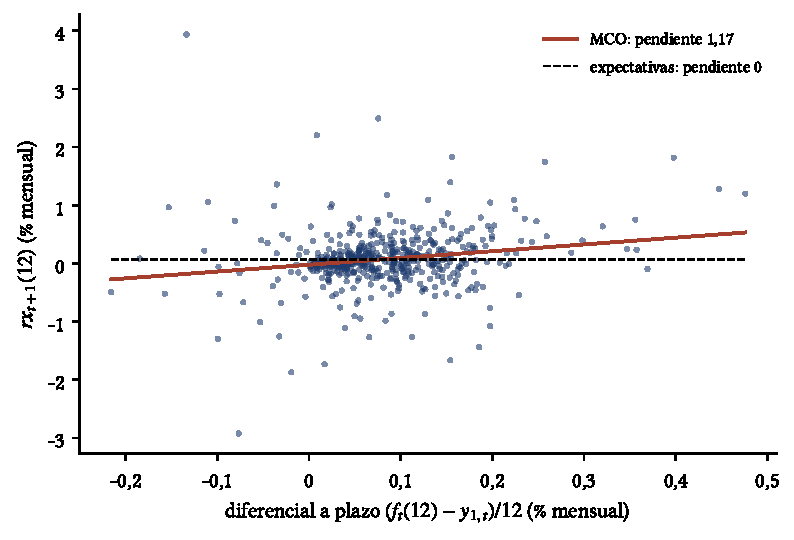
\includegraphics[width=0.75\linewidth]{graficos/cap15_ej03_fama_bliss.pdf}
\caption{Rendimiento en exceso del bono de 12 meses frente al diferencial a plazo en el mes anterior, con la recta de MCO y la
predicción de la HE (pendiente cero).}
\label{fig:fb}
\end{figure}

\begin{conclusion}
Comprar bonos cuando la tasa a plazo está alta respecto de la tasa corta fue, en promedio, rentable. Es la otra cara del
rechazo de la HE en el Ejercicio~\ref{ej:he}: la tasa a plazo contiene una prima de riesgo que varía en el tiempo, no solo
el pronóstico de la tasa futura.
\end{conclusion}
\end{ejresuelto}

\begin{ejresuelto}{Nelson-Siegel dinámico}\label{ej:ns}
\enunciado Ajuste el modelo de Nelson-Siegel mes a mes por MCO de corte transversal: (a) con el $\lambda$ que minimiza la suma
total de errores cuadráticos en una malla de 0,010 a 0,200 con paso 0,0005, y (b) con $\lambda=0{,}0609$. Compare el ajuste, la
persistencia de los factores y su relación con el nivel, la pendiente y la curvatura empíricos.

\solucion
\paso{Paso 1. El parámetro $\lambda$.} El mínimo de la malla está en $\hat\lambda=0{,}1410$, que pone el máximo de la curvatura en
\begin{align*}
  \tau^* &= \frac{1{,}7933}{0{,}1410}\\
         &= 12{,}7\ \text{meses}.
\end{align*}
Con estos datos, cuyos plazos se concentran por debajo del año, el ajuste prefiere una joroba más temprana que la de
Diebold y Li (Figura~\ref{fig:nslambda}).

\paso{Paso 2. Ajuste y factores.}
\begin{center}\small
\begin{tabular}{@{}lrrrrrr@{}}
\toprule
 & \multicolumn{3}{c}{$\lambda=0{,}1410$} & \multicolumn{3}{c}{$\lambda=0{,}0609$} \\
\cmidrule(lr){2-4}\cmidrule(lr){5-7}
 & Media & $\hat\rho(1)$ & $\hat\rho(12)$ & Media & $\hat\rho(1)$ & $\hat\rho(12)$ \\
\midrule
$\hat\beta_0$ & 6,134 & 0,994 & 0,921 & 6,098 & 0,993 & 0,928 \\
$\hat\beta_1$ & $-1{,}328$ & 0,902 & 0,346 & $-1{,}190$ & 0,923 & 0,393 \\
$\hat\beta_2$ & 0,210 & 0,807 & 0,408 & 1,061 & 0,758 & 0,315 \\
\midrule
RECM global & \multicolumn{3}{c}{0,102} & \multicolumn{3}{c}{0,130} \\
\bottomrule
\end{tabular}
\end{center}
Tres parámetros por mes ajustan diez rendimientos con un error cuadrático medio de 10 a 13 puntos básicos. Los mayores
errores con $\lambda=0{,}0609$ están en el plazo de un mes (0,237) y en el de 36 meses (0,164). El nivel es casi tan persistente
como los propios rendimientos; la pendiente y la curvatura lo son menos, pero aun así mucho (autocorrelación mensual de 0,76 a 0,92).

\paso{Paso 3. Interpretación.} Con $\lambda=0{,}0609$:
\begin{align*}
  \operatorname{corr}(\hat\beta_0,\ y_{120}) &= 0{,}991,\\
  \operatorname{corr}(-\hat\beta_1,\ y_{120}-y_3) &= 0{,}984,\\
  \operatorname{corr}(\hat\beta_2,\ 2y_{36}-y_3-y_{120}) &= 0{,}702 .
\end{align*}
Los factores tienen exactamente la interpretación de la Proposición~\ref{prop:ns} (Figura~\ref{fig:nsfac}). La curvatura es
la peor medida por su proxy empírico, que usa solo tres plazos. En septiembre de 1981, cuando la curva subía hasta 15,9\,\% a 11 meses y bajaba a 15,1\,\% a diez años,
$\hat\beta_1=0{,}420$ es positivo (el tramo largo queda por debajo del corto) y $\hat\beta_2=8{,}597$ refleja una joroba pronunciada; la RECM de ese mes, 0,314, es la mayor de las tres fechas
de la Figura~\ref{fig:nsajuste}.

\codigoweb{cap15_ej04}
\salidaR{cap15_ej04_R.txt}
\lectura{cap15_ej04}

\RvsPy Con $\lambda$ fijo, las 531 regresiones de corte transversal se resuelven con un solo sistema: $\hat B'=(X'X)^{-1}X'Y'$, donde
$X$ es la matriz $10\times3$ de cargas. En Python la malla se redondea (\texttt{np.round(..., 4)}) porque \texttt{np.arange} con
paso decimal acumula errores de punto flotante y el mínimo podría imprimirse como 0,14099999. En R, \texttt{seq} no tiene
ese problema en esta escala.

\begin{figure}[ht]
\centering
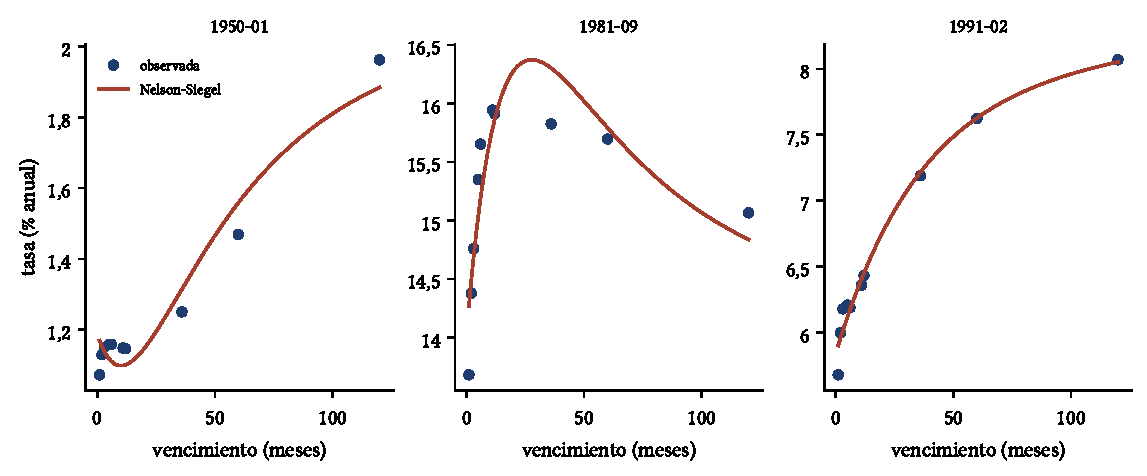
\includegraphics[width=\linewidth]{graficos/cap15_ej04_ajustes.pdf}
\caption{Curvas observadas (puntos) y ajustadas por Nelson-Siegel con $\lambda=0{,}0609$ en tres fechas: una curva baja y
creciente (1950), una con joroba y tramo largo descendente (1981) y una creciente al final de la muestra (1991).}
\label{fig:nsajuste}
\end{figure}

\begin{figure}[ht]
\centering
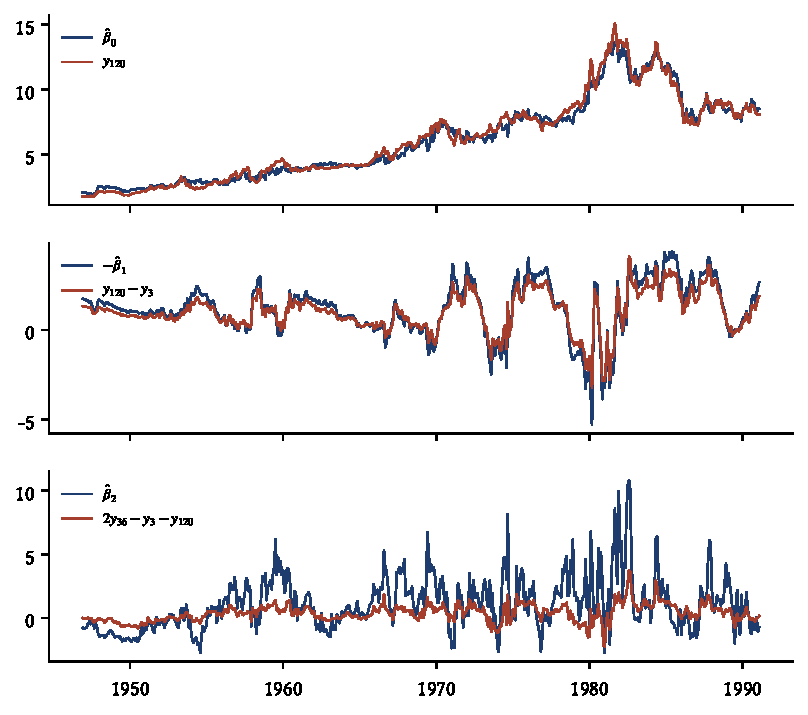
\includegraphics[width=0.85\linewidth]{graficos/cap15_ej04_factores.pdf}
\caption{Factores de Nelson-Siegel estimados (azul) y sus contrapartes empíricas (rojo): nivel, pendiente y curvatura.}
\label{fig:nsfac}
\end{figure}

\begin{figure}[ht]
\centering
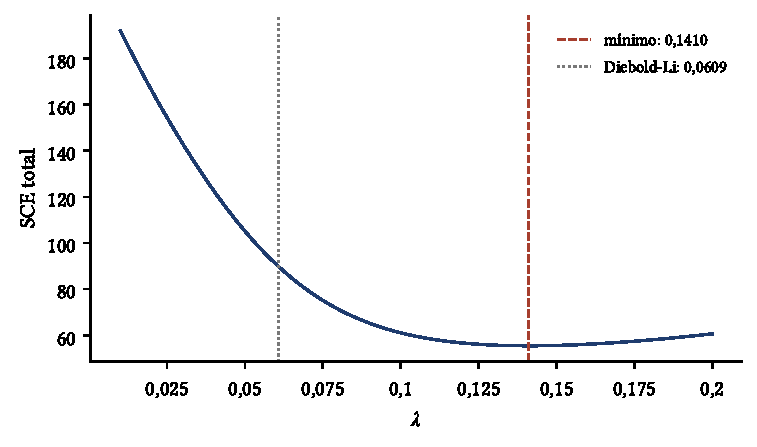
\includegraphics[width=0.7\linewidth]{graficos/cap15_ej04_lambda.pdf}
\caption{Suma de errores cuadráticos de todos los meses y vencimientos en función de $\lambda$.}
\label{fig:nslambda}
\end{figure}

\begin{conclusion}
El modelo de Nelson-Siegel dinámico logra con tres factores interpretables casi el mismo ajuste que los componentes
principales, pero con cargas suaves que permiten interpolar a cualquier plazo. Su $\lambda$ óptimo depende de los vencimientos
disponibles; fijarlo en 0,0609 cuesta poco en ajuste y facilita comparar con la literatura.
\end{conclusion}
\end{ejresuelto}

\begin{ejresuelto}{Vasicek y el efecto nivel}\label{ej:vasicek}
\enunciado Estime el modelo de Vasicek para la tasa a un mes con el AR(1) del Corolario~\ref{cor:vasicek} ($\Delta=1/12$
años). Calcule la vida media y la probabilidad estacionaria de tasas negativas. Luego contraste si la volatilidad depende
del nivel con la regresión de CKLS.

\solucion
\paso{Paso 1. El AR(1).} Por MCO, con $n=530$:
\[
  \hat a=0{,}10569\ (0{,}04752),\qquad \hat b=0{,}98016\ (0{,}00822),\qquad \hat s=0{,}60426 .
\]

\paso{Paso 2. Parámetros de Vasicek.}
\begin{align*}
  \hat\kappa &= -12\,\ln 0{,}98016\\
             &= -12\times(-0{,}020039)\\
             &= 0{,}2405\ \text{por año},\\[4pt]
  \hat\theta &= \frac{0{,}10569}{1-0{,}98016}\\
             &= \frac{0{,}10569}{0{,}01984}\\
             &= 5{,}327\text{\,\%},\\[4pt]
  1-\hat b^2 &= 1-0{,}960714\\
             &= 0{,}039286,\\
  \hat\sigma &= 0{,}60426\sqrt{\frac{2\times0{,}2405}{0{,}039286}}\\
             &= 0{,}60426\sqrt{12{,}243}\\
             &= 0{,}60426\times3{,}4991\\
             &= 2{,}114\text{\,\%}\ \text{por }\sqrt{\text{año}} .
\end{align*}
La vida media y la desviación estándar estacionaria son
\begin{align*}
  \frac{\ln2}{\hat\kappa} &= \frac{0{,}6931}{0{,}2405}\\
                          &= 2{,}88\ \text{años},\\[4pt]
  \frac{\hat\sigma}{\sqrt{2\hat\kappa}} &= \frac{2{,}114}{\sqrt{0{,}4809}}\\
                                         &= \frac{2{,}114}{0{,}6935}\\
                                         &= 3{,}049\text{\,\%}.
\end{align*}
La desviación estándar implícita (3,05) es parecida a la muestral (3,19), pero la media de largo plazo (5,33) está por encima
de la muestral (4,82): con una raíz tan cerca de uno, $\hat\theta$ es muy imprecisa. La probabilidad estacionaria de una tasa
negativa es $\Phi(-5{,}327/3{,}049)=0{,}040$, una de cada 25 observaciones, algo que nunca ocurrió en estos 44 años.

\paso{Paso 3. Efecto nivel.} La regresión de $\ln\hat e_t^2$ sobre $\ln r_{t-1}$ da
\begin{align*}
  2\hat\gamma &= 1{,}2787\ (0{,}1260)\\
  \hat\gamma  &= 0{,}639,\\
  t(\gamma=\tfrac12) &= \frac{1{,}2787-1}{0{,}1260}\\
                     &= 2{,}21 .
\end{align*}
Se rechaza $\gamma=0$ (Vasicek) con $t=10{,}15$, y también $\gamma=1/2$ (CIR) al 5\,\%. La desviación estándar de los residuos
lo muestra sin regresión: 0,273 cuando la tasa está en su tercil bajo (media 1,6\,\%), 0,330 en el medio (4,4\,\%) y 0,953 en el
alto (8,5\,\%) (Figura~\ref{fig:vasicekdatos}).

\codigoweb{cap15_ej05}
\salidaR{cap15_ej05_R.txt}
\lectura{cap15_ej05}

\RvsPy En R, \texttt{lm} entrega directamente los errores estándar; en Python escribimos la función \texttt{mco} con
$s^2(X'X)^{-1}$ para no depender de \texttt{statsmodels}. Los terciles se forman con \texttt{quantile} y
\texttt{np.quantile}, que usan
por omisión la misma interpolación (tipo 7), por eso los tamaños de los grupos (178, 175 y 177, desiguales por empates)
coinciden.

\begin{figure}[ht]
\centering
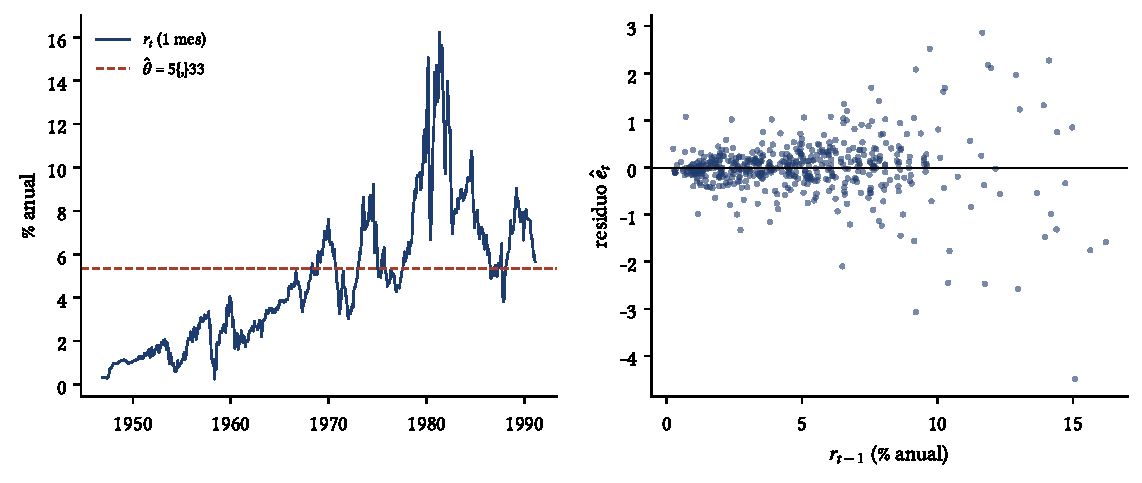
\includegraphics[width=\linewidth]{graficos/cap15_ej05_vasicek.pdf}
\caption{Izquierda: tasa a un mes y la media de largo plazo estimada por Vasicek. Derecha: residuos del AR(1) frente al
nivel del mes anterior; su dispersión crece con el nivel, en contra del supuesto de Vasicek.}
\label{fig:vasicekdatos}
\end{figure}

\begin{conclusion}
El modelo de Vasicek captura la reversión lenta de la tasa corta, pero su supuesto de volatilidad constante no se cumple: la
volatilidad crece con el nivel, con un exponente entre el de CIR y el de un proceso proporcional. Las conclusiones dependen
de la década de alta inflación y del experimento monetario de 1979--1982, como advierten CKLS.
\end{conclusion}
\end{ejresuelto}

% ---------------------------------------------------------------------
\section{Ejercicios propuestos}
% ---------------------------------------------------------------------

\begin{enumerate}[label=\textbf{\thechapter.\arabic*},leftmargin=*,itemsep=6pt]
  \item Con rendimientos compuestos en forma continua de 4\,\% a un año y 5\,\% a dos años, calcule la tasa a plazo entre el año
  1 y el 2, y el precio del bono cupón cero a cinco años si su rendimiento es 6\,\%. \textit{Respuesta: 6\,\%; $e^{-0{,}30}=0{,}7408$.}

  \item Con $\lambda=0{,}0609$ y $\boldsymbol\beta=(6;\,-2;\,1)$, calcule el rendimiento de Nelson-Siegel a 60 meses.
  \textit{Respuesta: las cargas son 0,2666 y 0,2407; $y(60)=5{,}708$\,\%.}

  \item Un AR(1) mensual de la tasa corta da $\hat a=0{,}15$, $\hat b=0{,}97$ y $\hat s=0{,}5$. Calcule $\kappa$, $\theta$, $\sigma$ y la
  vida media de Vasicek. \textit{Respuesta: $\kappa=0{,}3655$; $\theta=5$; $\sigma=1{,}758$; vida media $1{,}90$ años.}

  \item Demuestre que $y_{n,t}=\frac1n\sum_{i=1}^n f_t(i)$ y que, si la curva es creciente en $n$, entonces $f_t(n)\ge y_{n,t}$.

  \item Demuestre que, bajo la HE, la regresión de Fama y Bliss del cambio de la tasa corta,
  $y_{1,t+n-1}-y_{1,t}=a+b\,[f_t(n)-y_{1,t}]+u$, tiene $b=1$ cuando $n=2$.

  \item \emph{(Simulación.)} Simule 2\,000 muestras de 531 meses de un modelo de Vasicek con $\kappa=0{,}24$, $\theta=5{,}3$ y
  $\sigma=2{,}1$, y estime $\kappa$ en cada una con el Corolario~\ref{cor:vasicek}. ¿Cuál es el sesgo medio de $\hat\kappa$? Relaciónelo
  con el sesgo de Hurwicz de $\hat b$ (Capítulo~\ref{cap:raiz}).

  \item \emph{(Con datos del BCRP.)} Descargue de BCRPData los rendimientos de los bonos soberanos peruanos en soles en los
  plazos publicados (por ejemplo, 2, 5, 10, 15 y 20 años) y repita los Ejercicios~\ref{ej:curva} y \ref{ej:ns}. ¿Es el valor de $\lambda$ óptimo distinto del de Estados
  Unidos? ¿Por qué cabe esperarlo, si los plazos disponibles son otros?

  \item \emph{(Con datos.)} Repita el Ejercicio~\ref{ej:he} con dos submuestras: hasta septiembre de 1979 y desde octubre de 1979. ¿Se
  sostienen los resultados fuera del período de Volcker?
\end{enumerate}

% ---------------------------------------------------------------------
\section{Resumen de fórmulas}
% ---------------------------------------------------------------------

\begin{table}[H]
\centering\small
\begin{tabular}{@{}ll@{}}
\toprule
Concepto & Fórmula \\
\midrule
Precio y rendimiento & $P_{n,t}=e^{-n\,y_{n,t}}$;\quad $p_{n,t}=-n\,y_{n,t}$ \\
Tasa a plazo & $f_t(n,m)=\frac{m\,y_{m,t}-n\,y_{n,t}}{m-n}$;\quad $f_t(n)=n\,y_{n,t}-(n-1)\,y_{n-1,t}$ \\
Rendimiento en exceso & $rx_{t+1}(n)=[f_t(n)-y_{1,t}]-(n-1)[y_{n-1,t+1}-y_{n-1,t}]$ \\
HE: tasas cortas & $\frac1h\sum_{i=0}^{h-1}y_{m,t+mi}-y_{m,t}=a+b(y_{k,t}-y_{m,t})$;\quad $b=1$ \\
HE: tasa larga & $y_{n-1,t+1}-y_{n,t}=a+b\,\frac{y_{n,t}-y_{1,t}}{n-1}$;\quad $b=1$ \\
Fama-Bliss & $rx_{t+1}(n)=a+b\,[f_t(n)-y_{1,t}]$;\quad $b=0$ \\
Nelson-Siegel & $y(\tau)=\beta_0+\beta_1\frac{1-e^{-\lambda\tau}}{\lambda\tau}+\beta_2\bigl(\frac{1-e^{-\lambda\tau}}{\lambda\tau}-e^{-\lambda\tau}\bigr)$ \\
Vasicek exacto & $r_{t+\Delta}=\theta+e^{-\kappa\Delta}(r_t-\theta)+\varepsilon$;\quad $\Var(\varepsilon)=\sigma^2\frac{1-e^{-2\kappa\Delta}}{2\kappa}$ \\
Del AR(1) a Vasicek & $\kappa=-\ln b/\Delta$;\quad $\theta=a/(1-b)$;\quad $\sigma=s\sqrt{2\kappa/(1-b^2)}$ \\
CKLS & $dr=(\alpha+\beta r)\,dt+\sigma r^{\gamma}dW$;\quad $\ln\hat e^2_t\approx c+2\gamma\ln r_{t-1}$ \\
\bottomrule
\end{tabular}
\caption{Fórmulas principales del Capítulo 15.}
\end{table}

\section*{Referencias}
\begin{itemize}[leftmargin=*]
  \item Campbell, J. Y. y Shiller, R. J. (1991). Yield spreads and interest rate movements: A bird's eye view. \emph{Review of
        Economic Studies}, 58(3), 495--514.
  \item Chan, K. C., Karolyi, G. A., Longstaff, F. A. y Sanders, A. B. (1992). An empirical comparison of alternative models of
        the short-term interest rate. \emph{Journal of Finance}, 47(3), 1209--1227.
  \item Christensen, J. H. E., Diebold, F. X. y Rudebusch, G. D. (2011). The affine arbitrage-free class of Nelson-Siegel term
        structure models. \emph{Journal of Econometrics}, 164(1), 4--20.
  \item Cox, J. C., Ingersoll, J. E. y Ross, S. A. (1985). A theory of the term structure of interest rates. \emph{Econometrica},
        53(2), 385--407.
  \item Diebold, F. X. y Li, C. (2006). Forecasting the term structure of government bond yields. \emph{Journal of
        Econometrics}, 130(2), 337--364.
  \item Fama, E. F. y Bliss, R. R. (1987). The information in long-maturity forward rates. \emph{American Economic Review},
        77(4), 680--692.
  \item Litterman, R. y Scheinkman, J. (1991). Common factors affecting bond returns. \emph{Journal of Fixed Income}, 1(1),
        54--61.
  \item McCulloch, J. H. y Kwon, H.-C. (1993). U.S. term structure data, 1947--1991. Documento de trabajo, Ohio State University.
  \item Nelson, C. R. y Siegel, A. F. (1987). Parsimonious modeling of yield curves. \emph{Journal of Business}, 60(4), 473--489.
  \item Vasicek, O. (1977). An equilibrium characterization of the term structure. \emph{Journal of Financial Economics}, 5(2),
        177--188.
\end{itemize}
